\scanpage{210}
The system of groups \inserted{over $\mathbb{Q}$} (36, 37), equipped
with the homomorphism from
\[
\Pi \subset \mathcal{G} \subset M
\]
into \deleted{\unsure{$\mathcal{G}$}}
\[
(40)\qquad
\underline{\Pi}_{\mathbb{Q}}(\unsure{\mathbb{A}'_{\mathbb{Q}}})
\subset \underline{\mathcal{G}}_{\mathbb{Q}}(\mathbb{A}_{\mathbb{Q}})
\subset \underline{M}_{\mathbb{Q}}(\unsure{\mathbb{A}_{\mathbb{Q}}})
\]
\deleted{deduced} \inserted{induced} by
$M\longrightarrow \unsure{G}(\mathbb{A}_{\mathbb{Q}})$ (satisfying
conditions $1^\circ)$ to $4^\circ)$ above \deleted{\unsure{)}}, i.e.
of a ``Lie homomorphism'') will also be called
a ``\uline{Lie approximation}'' of the
Galois-Teichmüller system under consideration.

Consider a \deleted{germ of a }homomorphism
\[
(41)\qquad k_i^{\deleted{\unsure{\sharp}}}\quad T_0\longrightarrow\Pi_0
\]
\unsure{belonging|corresponding} to the L-structure of $\Pi$,
thus defines \inserted{by composition with
$\unsure{\Pi_0}\longrightarrow
\deleted{\unsure{\mathcal{G}}}\underline{\Pi}_{\deleted{\unsure{\mathbb{Q}}}}(\mathbb{Q})$}
a \deleted{germ of a }homomorphism
\[
(42)\qquad T_0\longrightarrow
\deleted{\unsure{\mathcal{G}}}\underline{\Pi}(\mathbb{Q}).
\]
\margin{\uline{N.B.} for fixed $i$,
$k_i$ is determined modulo
inner \unsure{automorphisms} of $\Pi_0$ \uuline{and}
modulo composition with
$n\,\mathrm{id}_{T_0}$, for $n\in\mathbb{N}^{*}$.
As for this last point, \unsure{there is}
\unsure{often} (\unsure{let us fix} $\Pi_0$) a
``best choice'', from which all \unsure{the others are}
deduced by composition with
$n\,\mathrm{id}_{T_0}$.}
We see \inserted{((21) page\,$747'$)} that this \deleted{germ of a} homomorphism
is quasi-unipotent, and that it therefore defines
a homomorphism of \deleted{\unsure{g}} group schemes
\margin{209}

\scanpage{211}
\mspage{753}
\[
(43)\qquad \underline{k}_i:
\underset{(\simeq G_{a\mathbb{Q}}\otimes_{\mathbb{Z}}T_0)}{\underline{T}_{0\mathbb{Q}}}
\longrightarrow \underline{\Pi}_{\mathbb{Q}}
\]
(not just a germ!)
which defines, by \deleted{composition} passage to
the $\mathbb{Q}$-rational points, the \uline{germ} of the homomorphism
(42). We thus find a finite set
(indexed by \inserted{the set} of germs of loop \uline{subgroups}
of $\Pi_0$, or of $\Pi$ which amounts \unsure{to the}
\unsure{same}) of outer homomorphisms (43) of group
schemes. I feel like calling the Lie appro-\deleted{\unsure{representation}}\inserted{ximation} \uline{nondegenerate} if
the preceding homomorphisms are all nontrivial,
hence are \uline{monomorphisms}.
\[
(44)\qquad \underline{k}_i:
\underline{T}_{0\mathbb{Q}}\simeq G_{a\mathbb{Q}}\otimes_{\mathbb{Z}}T_0
\lhook\joinrel\longrightarrow \underline{\Pi}_{\mathbb{Q}}.
\]

Suppose that $\underline{M}_{\mathbb{Q}}$ comes from
a group scheme (affine \unsure{and} of finite type)
$\underline{M}$ over $\mathbb{Z}$, such that we have
\[
(45)\qquad M\longrightarrow\underline{M}(\widehat{\mathbb{Z}})
\]
(it seems to me that one can always find
such an $\underline{M}$...). We then denote by
\margin{210}

\scanpage{212}
$\underline{\Pi}$, $\underline{\mathcal{G}}$ the schematic closures in
$\underline{M}$ of $\underline{\Pi}_{\mathbb{Q}}$, $\underline{\mathcal{G}}_{\mathbb{Q}}$, whence a diagram
of group schemes over $\mathbb{Z}$
\[
(46)\qquad
\diagram{\begin{tikzcd}[ampersand replacement=\&,column sep=3em]
\underline{\Pi}
\arrow[r,phantom,"\subset" description]
\arrow[r,no head,to path={(\tikztostart.north) -- ++(0,0.35) -| (\tikztotarget.north) \tikztonodes},"\underline{\unsure{\mathcal{T}}}"]
\arrow[rr,no head,to path={(\tikztostart.south) -- ++(0,-0.35) -| (\tikztotarget.south) \tikztonodes},"\underline{N}"']
\&\underline{\mathcal{G}}
\arrow[r,phantom,"\subset" description]
\arrow[r,no head,to path={(\tikztostart.north) -- ++(0,0.35) -| (\tikztotarget.north) \tikztonodes},"\underline{\Gamma}"]
\&\underline{M}
\end{tikzcd}}
\]
(subject to representability of the
quotients $\underline{\unsure{\mathcal{T}}}$, $\underline{\Gamma}$, $\underline{N}$ --- but I think that
for Raynaud there is never any problem...).
We \deleted{\unsure{are going to assume|assume} of course that}
\inserted{will have factorizations}
\[
(47)\qquad
\diagram{\begin{tikzcd}[ampersand replacement=\&,column sep=large,row sep=large]
\Pi_0\arrow[r,hook,no head]\arrow[d]
\&\mathcal{G}_0\arrow[r,hook]\arrow[d]
\&M\arrow[d]\\
\underline{\Pi}(\mathbb{Z})\arrow[r,hook]
\&\underline{\mathcal{G}}(\mathbb{Z})\arrow[r,hook,no head]
\&\underline{M}(\widehat{\mathbb{Z}}).
\end{tikzcd}}
\]

We assume of course \deleted{\unsure{(is there}} that
the homomorphism $\chi_{\underline{\unsure{M}}}:\deleted{\unsure{\mathbb{Q}}}\underline{M}_{\mathbb{Q}}\longrightarrow G_{m\mathbb{Q}}$
extends to
\[
(48)\qquad \chi_{\underline{M}}:\underline{M}\longrightarrow G_{m\mathbb{Z}},
\]
which obviously factors through
\[
(49)\qquad \chi_{\underline{\Gamma}}:\underline{\Gamma}\longrightarrow G_{m\mathbb{Z}}.
\]
\margin{211}


\scanpage{213}
\mspage{754}
It would be interesting to bring out a theorem of existence,
(or \inserted{\unsure{even}} of uniqueness, under still stronger conditions)
of a ``model'' $\underline{M}$ \inserted{\uline{smooth}} over $\mathbb{Z}$ of $\underline{M}_{\mathbb{Q}}$,
satisfying the preceding conditions
\figure{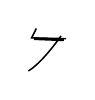
\begin{tikzpicture}[x=0.5cm,y=0.5cm,baseline=0]
\draw[line width=0.55pt] (0.12,0.72)--(0,0.48)--(0.88,0.46);
\draw[line width=1pt] (0.06,0.46)--(0.82,0.43);
\draw[line width=0.55pt] (0.75,0.53) .. controls (0.48,0.16) and (0.18,-0.2) .. (-0.08,-0.36);
\end{tikzpicture}}
\[
(M\longrightarrow\underline{M}(\mathbb{Z}),\quad
\text{and }\underline{M}\xrightarrow{\chi_{\underline{M}}}G_{m\mathbb{Z}}).
\]

Here it will no longer be true in general, I
presume, that the outer homomorphisms \inserted{$\underline{k}_i$} (43)
extend as they stand to homomorphisms
$\underline{T}_i\underset{\unsure{\mathrm{df}}}{=}\underline{T}_{i\mathbb{Z}}\longrightarrow\underline{\Pi}$.
But I \unsure{am going to|have one} consider
the centralizer of $k_i:T_0\longrightarrow\Pi_0$ in $\Pi_0$,
i.e. $\widetilde{L}_{i,0}$ which is a
metabelian group: $\operatorname{Im}(T_0\xrightarrow{k_i}\Pi_0)$ is a
\inserted{normal} subgroup of finite index in it. Consider
the homomorphism
\[
(50)\qquad
\diagram{\begin{tikzcd}[ampersand replacement=\&,column sep=large,row sep=small]
\widetilde{L}_{i,0}\arrow[r]\arrow[d,equal]
\&\underline{\Pi}(\mathbb{Z}),\\
\operatorname{Centr}_{\Pi_0}(k_i:T_0\longrightarrow\Pi_0)\&
\end{tikzcd}}
\]
which is \unsure{entirely} unipotent --- it therefore factors
through a homomorphism of group schemes
\[
(51)\qquad \operatorname{Env}(\widetilde{L}_{i,0})\longrightarrow\underline{\Pi}
\]
(cf.\ \S\,50, $4^\circ$, page\,$658'$ ff), factoring
\margin{212}


\scanpage{214}
through one of the smooth \unsure{quotient|quotients} group \inserted{schemes} \inserted{$\underline{Z}_{i,n}$} of
$\operatorname{Env}(\widetilde{L}_{i,0})$, of which the latter is the $\varprojlim$:
\[
(52)\qquad
\diagram{\begin{tikzcd}[ampersand replacement=\&,column sep=large,row sep=small]
1\arrow[r,no head]\&\underline{nT_0}\arrow[r]
\&\underline{Z}_{i,n}\arrow[r]
\&(H_{i,n})_{S_0}\arrow[r,no head]\arrow[d,phantom,"\simeq"{description,rotate=90}]
\&1\\
\&\&\& (\widetilde{L}_{i,0}/nT_0)\&
\end{tikzcd}}
\]
\margin{$S_0=\operatorname{Spec}\mathbb{Z}$}
But of course, the restriction of the homomorphism
obtained
\[
\unsure{(5|(s}\qquad \underline{Z}_{i,n}\longrightarrow\underline{\Pi}
\]
to
\[
\underline{Z}_{i,n}^{\circ}\simeq\underline{nT_0}
\]
is not in general a monomorphism --- if it
is for fixed $n$, then if $n\mid n'$, $n\ne n'$,
it no longer is for $n'$. A particularly
favorable case would be one where
one can find $n$ such that the induced
homomorphism
\[
(53)\qquad\underline{nT_0}\longrightarrow\underline{\Pi}
\]
\margin{this $n$ is then \uline{unique}.}
is a monomorphism. This implies that the schematic
closure in $\underline{\Pi}$ of the ``$1$-parameter
additive subgroup''
$\deleted{\unsure{\mathcal{G}}}\underline{L}_{i\mathbb{Q}}
=\underline{k}_i(\underline{\unsure{T_0}})$
is a \uline{smooth} subgroup scheme of $\underline{\Pi}$.
\margin{213}

\scanpage{215}
\mspage{755}

This condition should also be sufficient -- at least if one requires that this schematic closure have an identity component which is $\unsure{=|\simeq}$ isomorphic to $\mathrm{G}_{aS_0}$.
We then find, \inserted{in any case,} a unique \uline{monomorphism} (up to conjugation)
\[
(54)\qquad \deleted{\unsure{k}}\uuline{k_i'}:\quad
\diagram{\begin{tikzcd}[ampersand replacement=\&,column sep=large]
\underline{T_0} \arrow[r,hook] \& \underline{\Pi}
\end{tikzcd}}
\]
such that $\uuline{k_i'}_{\mathbb{Q}}$ is of the form $\underline{k_i}_{\mathbb{Q}}\circ(\unsure{r_i}\mathrm{id})$,
\deleted{for}\inserted{with} a suitable $\unsure{\parallel|!!}\ \unsure{r_i}\in\mathbb{Q}^{*+}$.
I am not sure that under these conditions, \deleted{one \unsure{can} find a} \inserted{the }homomorphism deduced from $\underline{k_i'}$ by passing to the $\mathbb{Z}$-points
\[
\diagram{\begin{tikzcd}[ampersand replacement=\&,column sep=large]
T_0\simeq\underline{T_0}(\mathbb{Z}) \arrow[r] \& \underline{\Pi}(\mathbb{Z})
\end{tikzcd}}
\]
factors into a homomorphism
\[
(55)\qquad
\diagram{\begin{tikzcd}[ampersand replacement=\&,column sep=large]
T_0 \arrow[r,"{k_i'\unsure{\varphi|?}}"] \& \Pi_0 \arrow[r,"{\mathrm{can}}"] \& \underline{\Pi}(\mathbb{Z})
\end{tikzcd}},
\]
\unsure{where} $T_0\longrightarrow\Pi_0$ \unsure{belongs} to the \uline{``germ''} $\underline{k_i}$, ---

I will nevertheless take it as an \inserted{additional} hypothesis, when the $\underline{k_i'}$ exist.

I feel like stating a few other ``good hypotheses'', which we will try to \unsure{realize}
\margin{214}

\scanpage{216}

in working on ``integral'' Lie approximations i.e. over $\operatorname{Spec}\mathbb{Z}$.

Consider all possible homomorphisms $\underline{k_i'}$ ($i$ variable, but also by conjugating the original $k_i:\deleted{\unsure{T_0}}\ T_0\longrightarrow\Pi_0$ by arbitrary elements of $\Pi_0$), and the corresponding homomorphisms on the Lie algebras
\[
(56)\qquad \operatorname{Lie}(\underline{k_i'}):\quad
\diagram{\begin{tikzcd}[ampersand replacement=\&,column sep=large,row sep=small]
\deleted{\unsure{\mathbb{Z}}}\ T_0 \arrow[r] \arrow[d,phantom,"{\wr}" description] \& \Gamma\underline{\operatorname{Lie}}(\underline{\Pi})\underset{\unsure{\mathrm{df}}}{=}\operatorname{Lie}(\underline{\Pi}) \\
\begin{gathered}\mathbb{Z}\\\text{(not canonical)}\end{gathered} \&
\end{tikzcd}}
\]
which \unsure{are} by hypothesis \deleted{\unsure{good|a}} universal monomorphisms, we would like $\Gamma\underline{\operatorname{Lie}}(\underline{\Pi})$ to be \uline{generated} (as a $\mathbb{Z}$-module) by their images, or (\unsure{that} which amounts to the same) by the images of a generator of $T_0$.
\margin{this hypothesis \unsure{seems} reasonable in a case like $\Pi_0=\operatorname{SL}(2,\mathbb{Z})$, but \unsure{not if} $I=\varnothing$ for example\ldots !}
\unsure{It|I} amounts to the same to say that if one chooses for $\forall i$ \uline{one} $\underline{k_i'}$, whence the image \inserted{in $\Gamma\underline{\operatorname{Lie}}(\underline{\Pi})$} of a generating element of $T_0$, the $I$ elements obtained in $\deleted{\unsure{\Gamma}}\operatorname{Lie}(\underline{\Pi})$, \uline{and} their conjugates by the elements of $\Pi_0$, generate the $\mathbb{Z}$-module $\operatorname{Lie}(\underline{\Pi})$. This \deleted{means} implies that
\margin{215}